\section{Introduction}
\textit{\say{... You took my sonar concept and applied it to every phone in the city. With half the city feeding you sonar, you can image all of Gotham.}} - \textit{Lucious Fox, The Dark Knight.}\\

When in the movie \textit{The Dark Knight}, \textit{Lucious Fox} mentioned the above dialogue to \textit{Batman}, \textit{Batman} was then trying to locate \textit{Joker} to save the city of \textit{Gotham}. There, \textit{Batman} used the smartphones of people to use them as audio based imaging devices (based on the principle of sonar). It helped him to get real-time information about different events happening around the city. Interestingly, the idea of sonar stems from the \textit{echolocation} cite{XXX} which bats or dolphins use to move in the dark or to catch their prey. \textit{Echolocation} is a biological mechanism used to detect and locate objects by emitting usually high-pitched sounds that reflect off the object and carefully \textit{listening} (via ears or other sensory receptors) to the different echoes. In this paper, we ask that can we give this superpower to humans through a smartphone ? Can we really \textit{hear} the visual characteristics of our surrounding ? Can we just \textit{plug and play} the mechanism of sonar \ie echo based location technique to get the information ? \\

In this paper, while answering the above questions, we attempt to see how much of this \textit{grand vision} can be achieved with our current smartphone without any external component or modification. We envision to map the surrounding with a smartphone using emitted and reflected audio signals.  As a first step in that direction, specifically, we use smartphone to infer $2D$ contour or shape skeleton of a room. We build a system called \textit{BatPhone}, which user employs to get the shape of the room by moving around the room. To achieve this, our \textit{Batphone} system utilizes FMCW radar based technology combined with IMU sensor based dead-reckoning. It also exploits the geometric constraints of the user movement and the room shape to construct an accurate room shape profile. Furthermore, we use specific reflection profile of FMCW chirps to detect different points of interest like corners or wall intersections, which are critical for accurate profile. \\

In general, there is a recent surge of interest in industry to get structural information about the surrounding of a user. The reason is to enrich the augmented reality (AR) or virtual reality (VR) applications cite{XXX}. If these applications get accurate $3D$ or $2D$ mapping of the surrounding, they can provide more realistic and engaging experience to users. People can play AR games which can seamlessly blend with the surrounding (\eg a spacecraft on a living room floor or an alien insect on a wall). Even VR experience becomes far smoother if it makes user aware of the surrounding cite{XXX}. To achieve this, there are multi-camera and multi-depth sensor based solutions like Microsoft Hololens, Google's Project Tango tablet, Oculus VR headset etc. Unfortunately, this solution are costly and requires user to buy a separate device. So, our solution holds promise to provide cheap, device-free technique to get $2D$ mapping or depth information by utilizing built-in speaker and microphone of a smartphone. Furthermore, \textit{Batphone} can help to create different interesting use-cases like navigation app for blind people, an app for creating $3D$ picture using image and depth information, enriching information for AR/VR applications etc. (as illustrated in Fig. ~\ref{fig:apps}).\\

\begin{figure*}[hbt]

\subfigure[]{
    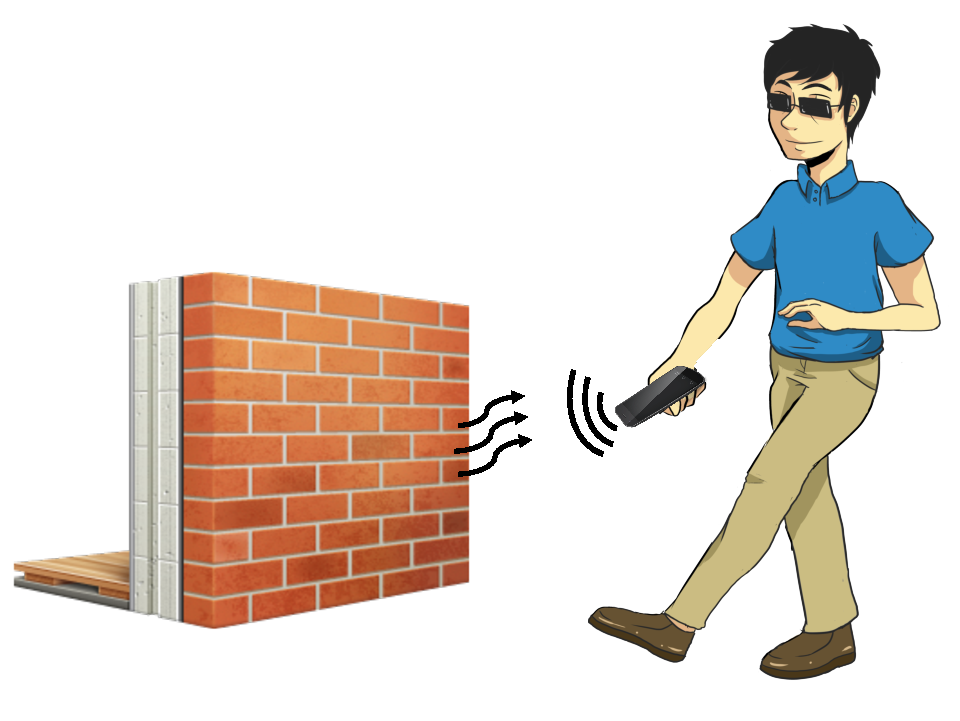
\includegraphics[width=0.32\textwidth, keepaspectratio]{figs/BlindPerson.pdf}
    \label{fig:app_blind}
}
\subfigure[]{
    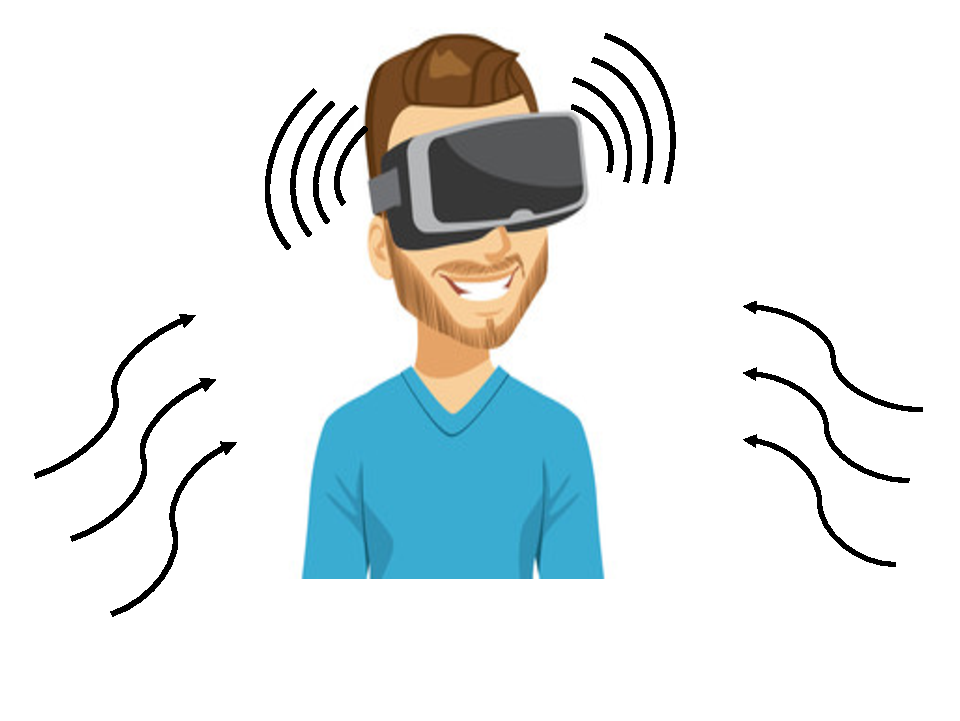
\includegraphics[width=0.32\textwidth, keepaspectratio]{figs/vrapp_another.pdf}
    \label{fig:app_vr}
}
\subfigure[]{
    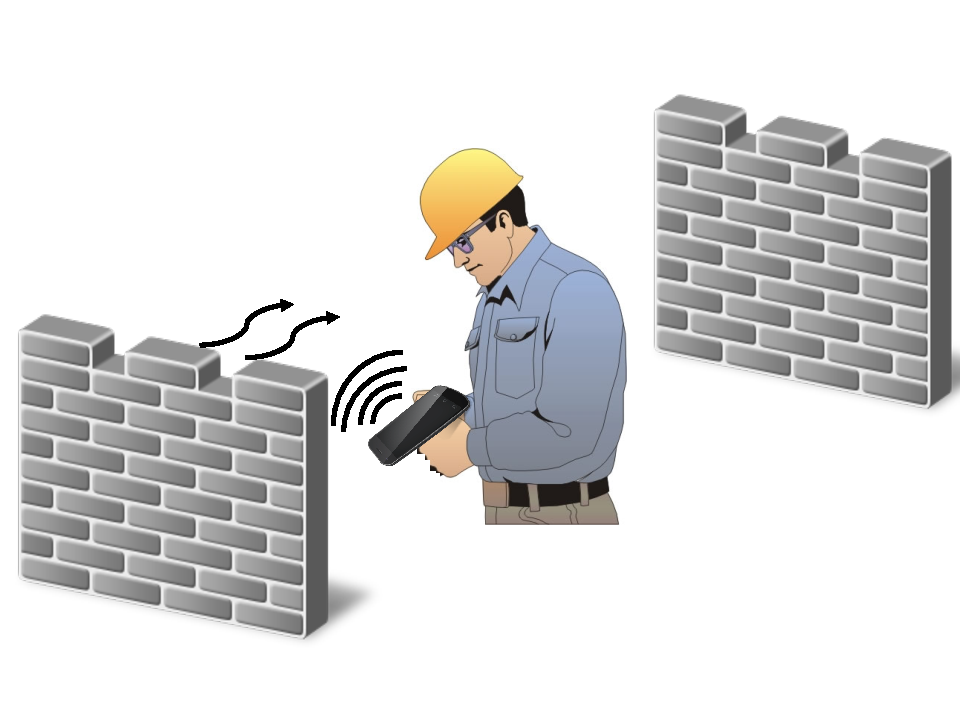
\includegraphics[width=0.32\textwidth, keepaspectratio]{figs/Engg.pdf}
    \label{fig:app_engg}
}

\caption{{\small (a). Blind Person Obstacle Detection App. (b). AR/VR application. (c). Helping in construction mapping. }}
%\vspace{-0.15in}
\label{fig:apps}

\end{figure*}
 
Recently, researchers have become interested to use acoustic signals to build different tracking, gesture detection, or activity recognition applications cite{XXX}. This immense popularity of audio based applications is due to its easy implementation or prototyping. It is also due to the relative low speed of propagation and low sampling rate of audio signal compared to other high-frequency wireless signals. In general, there is no need of any hardware modification in current infrastructure. Therefore, these applications are easy-to-scale and cheap to implement. There are two basic threads of work are coming out of the research community : device-free mechanism and device-based mechanism. In device-based mechanism, the audio source and the receiver are different and for the device-free technique, the source and the receiver are collocated. In device-based mechanism, audio source like speaker emits specific audio chirps and mic of the device like smartphone pick up that sound to analyze different properties like time-of-flight, phase cite{XXX} etc. Sometimes, the device collect these information from the emitted signal of multiple speakers at different locations to localize accurately cite{XXX, tonetrack,DopEnc}. In device-free mechanism, researchers use smartphone or smartwatch as transreceiver and pick up the movements of finger or hand. Authors have also exploited doppler based frequency change, FMCW chirp based frequency change, or channel impulse response estimation based techniques cite{XXX} to track fine-grained movement in presence of varying degree of multi-path. In both of the schemes, unsurprisingly, smartphones are used as the central device to render the application.\\ 

To the best of our knowledge, we are first to propose a single step infrastructure-free smartphone based acoustic mapping solution which does not depend upon any crowd-sourcing or multiple trials by same user. In this paper, as a first step to build an acoustic based indoor mapping solution, we attempt to make a $2D$ contour of a closed or semi-closed space. To achieve this, firstly we analyze the capability of the mics and speakers current smartphone which may be critical in this application. We carefully investigate different trade-offs involved in designing a light-weight calibration-free solution which suits the purpose. Secondly, we borrow the principle of RADAR citeXXX technology based on Frequency Modulated Continuous Wave (FMCW) technology to calculate the distances from the walls to user. We also show why the echo-based method citeXXX or channel impulse response (CIR) based methods are difficult to use in this problem, specifically in a calibration-free single-step setting. We carefully look at the challenges involved in multi-path heavy indoor environment and reflection dominant (resulting in numerous echoes) audio signals, to achieve that goal. It is important to point out that, all the audio based tracking related works \cite{fingerio,aamouse,cat} cancel out the static multi-path by taking difference of consecutive samples. Whereas we exploit this multi-path which indirectly manifests itself in the FMCW profile to get critical structural information like corner or clutter. Furthermore, we employ customized IMU-based dead-reckoning combined with these distance measurements and systematic geometric constraints to derive different surrounding shape information. We slowly build from a single wall scenario to multi-wall setting in the presence of static clutter. We also show that with other possible \textit{easy-to-attach} extensions to the smartphone, we can make the system faster and more light-weight. Finally, we demonstrate the strength of our core technology through a set of applications. \\
 
Our main contributions are the following:
\begin{itemize}
\item We measured in detail the building blocks necessary to design a infrastructure-free, calibration-free, and device-free acoustic mapping solution. Specifically, we focus on exploring different parameters, and trade-offs of a FMCW-based distance measurement scheme, which is particularly suitable for mapping, on a smartphone .
\item We developed a novel algorithm which can construct the contour of any indoor space around a user with a smartphone in a calibration-free manner.
\item We also build an \textit{end-to-end} system using our algorithm which intelligently combines IMU-based dead-reckoning and FMCW-based surrounding profiling, to construct the contour of an indoor space around a user.
\end{itemize}

Section Description.\\

 
 
 
 
